\section{1174004 - Choirulanam}
\subsection{Data Types}
	\hfill\break
	Tipe data Struktur paling signifikan dalam Python adalah list, tupel, dan dictionary. Set telah diintegrasikan ke dalam Python sejak versi 2.5 (versi sebelumnya tersedia di perpustakaan set): List: Ini mirip dengan array satu dimensi, tetapi Anda dapat membuat daftar yang berisi daftar lain. Dictionary: Ini adalah array yang berisi pasangan kunci dan nilai-nilai (tabel hash). Tuples: Ini adalah objek mono-dimensi abadi. Array dapat berupa jenis apa saja, sehingga Anda dapat mencampur variabel seperti bilangan bulat dan string ke dalam daftar, kamus, dan tupel Anda. Indeks objek pertama dalam semua jenis array selalu nol. Indeks negatif diizinkan dan dihitung dari akhir array; -1 menunjukkan elemen terakhir dari array:

	\begin{itemize}
		\item Contoh List
		\hfill\break
	           \lstinputlisting[firstline=7, lastline=11]{src/kelompok1/srcsistemtersebar.py}
		\hfill\break
		dan berikut hasilnya:
		\begin{figure}[H]
		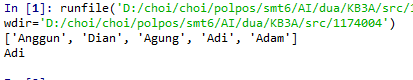
\includegraphics[width=4cm]{figures/kelompok1/1/anam/list.png}
		\centering
		\caption{List}
		\end{figure}

		\item Contoh Dictionary
		\hfill\break
	           \lstinputlisting[firstline=13, lastline=17]{src/kelompok1/srcsistemtersebar.py}
		\hfill\break
		dan berikut hasilnya:
		\begin{figure}[H]
		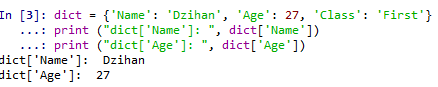
\includegraphics[width=4cm]{figures/kelompok1/1/anam/dict.png}
		\centering
		\caption{Dictionary}
		\end{figure}

		\item Contoh Tuple
		\hfill\break
	           \lstinputlisting[firstline=19, lastline=25]{src/kelompok1/srcsistemtersebar.py}
		\hfill\break
		dan berikut hasilnya:
		\begin{figure}[H]
		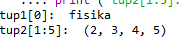
\includegraphics[width=4cm]{figures/kelompok1/1/anam/tupl.png}
		\centering
		\caption{Tuple}
		\end{figure}
	\end{itemize}

\subsection{String}
	\hfill\break
	String python diindikasikan menggunakan tanda kutip tunggal (') atau ganda (") dan diizinkan menggunakan satu notasi dalam string yang dibatasi oleh yang lain:
	\begin{itemize}
		\item Contoh String
		\hfill\break
	           \lstinputlisting[firstline=27, lastline=34]{src/kelompok1/srcsistemtersebar.py}
		\hfill\break
		dan berikut hasilnya:
		\begin{figure}[H]
		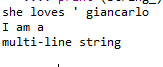
\includegraphics[width=4cm]{figures/kelompok1/1/anam/string.png}
		\centering
		\caption{String}
		\end{figure}
	\end{itemize}

\subsection{Bukti Tidak Plagiat}
\begin{figure}[H]
	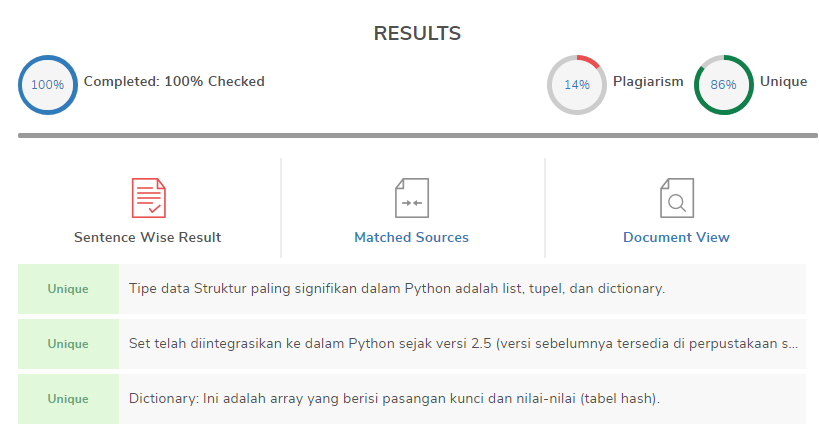
\includegraphics[width=4cm]{figures/kelompok1/1/anam/plagiat_anam.png}
	\centering
	\caption{Bukti Tidak Melakukan Plagiat Chapter 1}
\end{figure}

\section{1174012 - Damara Benedikta}
\subsection{Flow control }
Flow control merupakan sebuah pengelolaan (data flow) atau aliran data antara komputer atau perangkat atau antar node dalam suatu jaringan sehingga data dapat ditangani dengan kecepatan yang efisien.
Dimana terdapat if, for dan while. Terdapat dua jenis perualangan dalam bahasa pemrograman python, yaitu perulangan dengan for dan while
Perulangan for disebut counted loop (perulangan yang terhitung), sementara perulangan while disebut uncounted loop (perulangan yang tak terhitung). Perbedaannya adalah perulangan for biasanya digunakan untuk mengulangi kode yang sudah diketahui banyak perulangannya. Sementara while untuk perulangan yang memiliki syarat dan tidak tentu berapa banyak perulangannya.
Serta Kondisi If Pengambilan keputusan (kondisi if) digunakan untuk mengantisipasi kondisi yang terjadi saat jalanya program dan menentukan tindakan apa yang akan diambil sesuai dengan kondisi.
\hfill\break
\lstinputlisting[firstline=8, lastline=21]{src/kelompok1/perulangan.py}
\hfill\break

	\begin{figure}[H]
		\centering
		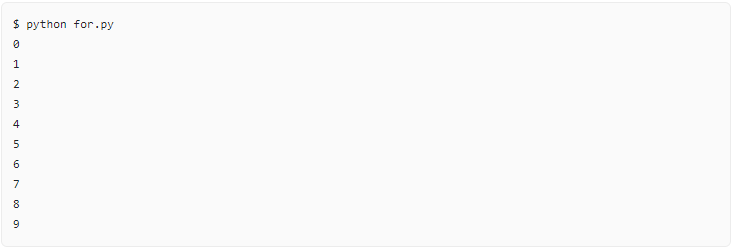
\includegraphics[width=4cm]{figures/kelompok1/1/damara/o_for.PNG}
		\caption{contoh perulangan for}
	\end{figure}

	\begin{figure}[H]
		\centering
		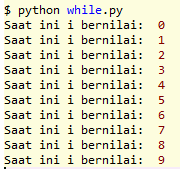
\includegraphics[width=4cm]{figures/kelompok1/1/damara/o_while.PNG}
		\caption{contoh perulangan while}
	\end{figure}

\subsection{Functions}
Fungsi adalah bagian dari program yang dapat digunakan ulang. Hal ini bisa dicapai dengan memberi nama pada blok statemen, kemudian nama ini dapat dipanggil di manapun dalam program. Kita telah menggunakan beberapa fungsi builtin seperti range.
Fungsi dalam Python didefinisikan menggunakan kata kunci def. Setelah def ada nama pengenal fungsi diikut dengan parameter yang diapit oleh tanda kurung dan diakhir dingan tanda titik dua 
\hfill\break
\lstinputlisting[firstline=23, lastline=44]{src/kelompok1/perulangan.py}
\hfill\break
\subsection{Bukti Tidak Plagiat}
\begin{figure}[H]
\centering
	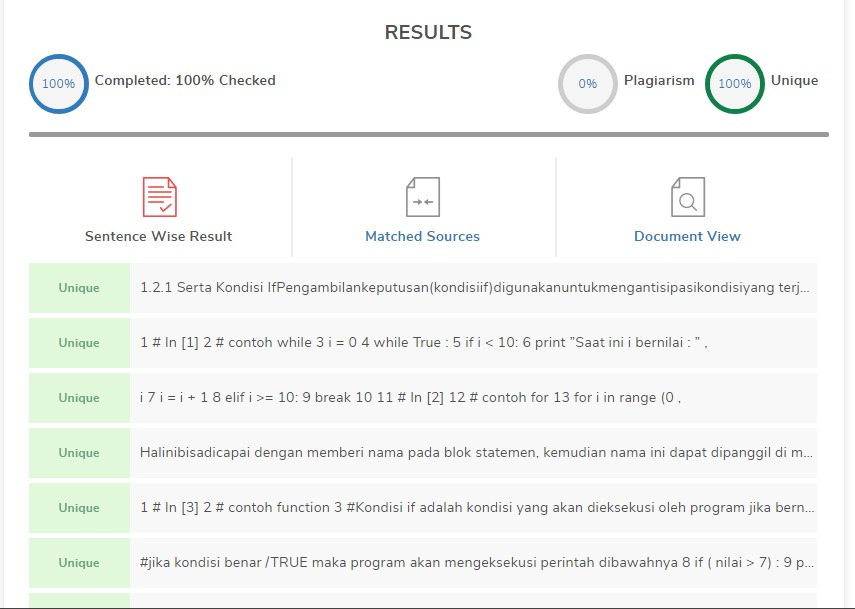
\includegraphics[width=4cm]{figures/kelompok1/1/damara/plagiat.jpeg}
	\caption{Bukti Tidak Melakukan Plagiat Chapter 1}
\end{figure}

\section{1174095 - Muhammad Dzihan}
\subsection{Class}
Python mendukung banyak warisan kelas. Secara konvensional (bukan aturan bahasa), variabel dan metode pribadi dideklarasikan dengan didahului dengan dua garis bawah. Kita dapat menetapkan atribut (properti) yang berubah-ubah ke instance kelas, seperti yang ditunjukkan pada contoh berikut:
\hfill\break
\lstinputlisting[firstline=7, lastline=16]{src/kelompok1/class.py}

\hfill\break
	\begin{figure}[H]
		\centering
		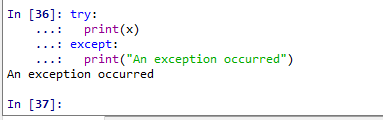
\includegraphics[width=4cm]{figures/kelompok1/1/dzihan/class1.PNG}
		\caption{Exceptions1}
	\end{figure}
\hfill\break
\lstinputlisting[firstline=17, lastline=20]{src/kelompok1/class.py}

\hfill\break
	\begin{figure}[H]
		\centering
		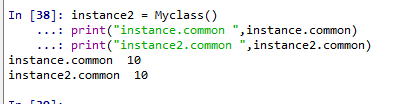
\includegraphics[width=4cm]{figures/kelompok1/1/dzihan/class2.PNG}
		\caption{Exceptions2}
	\end{figure}
\hfill\break
\lstinputlisting[firstline=21, lastline=26]{src/kelompok1/class.py}

\hfill\break
	\begin{figure}[H]
		\centering
		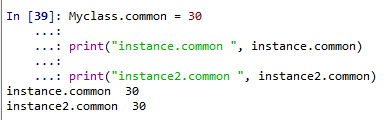
\includegraphics[width=4cm]{figures/kelompok1/1/dzihan/class3.PNG}
		\caption{Exceptions3}
	\end{figure}
\hfill\break
\lstinputlisting[firstline=27, lastline=31]{src/kelompok1/class.py}

\hfill\break
	\begin{figure}[H]
		\centering
		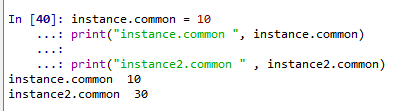
\includegraphics[width=4cm]{figures/kelompok1/1/dzihan/class4.PNG}
		\caption{Exceptions4}
	\end{figure}
\hfill\break
\lstinputlisting[firstline=32, lastline=36]{src/kelompok1/class.py}

\hfill\break
	\begin{figure}[H]
		\centering
		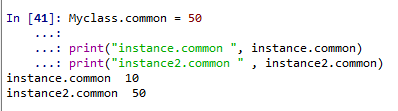
\includegraphics[width=4cm]{figures/kelompok1/1/dzihan/class5.PNG}
		\caption{Exceptions5}
	\end{figure}
\hfill\break
\lstinputlisting[firstline=37, lastline=47]{src/kelompok1/class.py}

\hfill\break
	\begin{figure}[H]
		\centering
		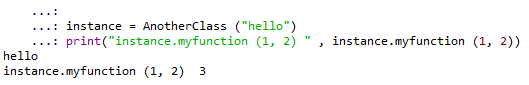
\includegraphics[width=4cm]{figures/kelompok1/1/dzihan/class6.PNG}
		\caption{Exceptions6}
	\end{figure}
\hfill\break
\lstinputlisting[firstline=48, lastline=51]{src/kelompok1/class.py}

\hfill\break
	\begin{figure}[H]
		\centering
		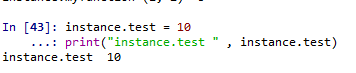
\includegraphics[width=4cm]{figures/kelompok1/1/dzihan/class7.PNG}
		\caption{Exceptions7}
	\end{figure}
\subsection{Exceptions}
Exceptions adalah peristiwa yang terjadi selama pelaksanaan program yang mengganggu aliran normal instruksi program. Secara umum, ketika skrip Python menemukan situasi yang tidak dapat diatasi, itu menimbulkan pengecualian. Pengecualian adalah objek Python yang mewakili kesalahan.
\hfill\break
\lstinputlisting[firstline=7, lastline=11]{src/kelompok1/exception.py}
\hfill\break
	\begin{figure}[H]
		\centering
		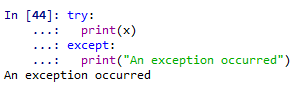
\includegraphics[width=4cm]{figures/kelompok1/1/dzihan/exc1.PNG}
		\caption{Exceptions1}
	\end{figure}
\hfill\break
\lstinputlisting[firstline=12, lastline=18]{src/kelompok1/exception.py}
\hfill\break
	\begin{figure}[H]
		\centering
		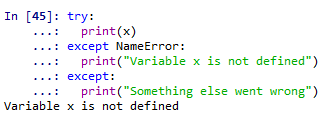
\includegraphics[width=4cm]{figures/kelompok1/1/dzihan/exc2.PNG}
		\caption{Exceptions2}
	\end{figure}
\hfill\break
\lstinputlisting[firstline=19, lastline=25]{src/kelompok1/exception.py}
\hfill\break
	\begin{figure}[H]
		\centering
		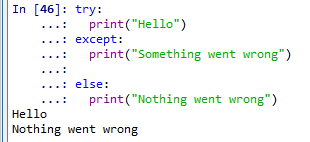
\includegraphics[width=4cm]{figures/kelompok1/1/dzihan/exc3.PNG}
		\caption{Exceptions3}
	\end{figure}
\hfill\break
\lstinputlisting[firstline=26, lastline=32]{src/kelompok1/exception.py}
\hfill\break
	\begin{figure}[H]
		\centering
		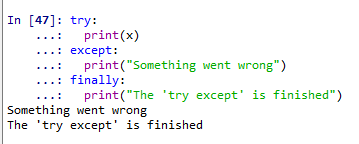
\includegraphics[width=4cm]{figures/kelompok1/1/dzihan/exc4.PNG}
		\caption{Exceptions4}
	\end{figure}
\hfill\break
\lstinputlisting[firstline=33, lastline=40]{src/kelompok1/exception.py}
\hfill\break
	\begin{figure}[H]
		\centering
		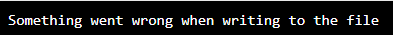
\includegraphics[width=4cm]{figures/kelompok1/1/dzihan/exc5.PNG}
		\caption{Exceptions5}
	\end{figure}

\subsection{Bukti Tidak Plagiat}
\begin{figure}[H]
\centering
	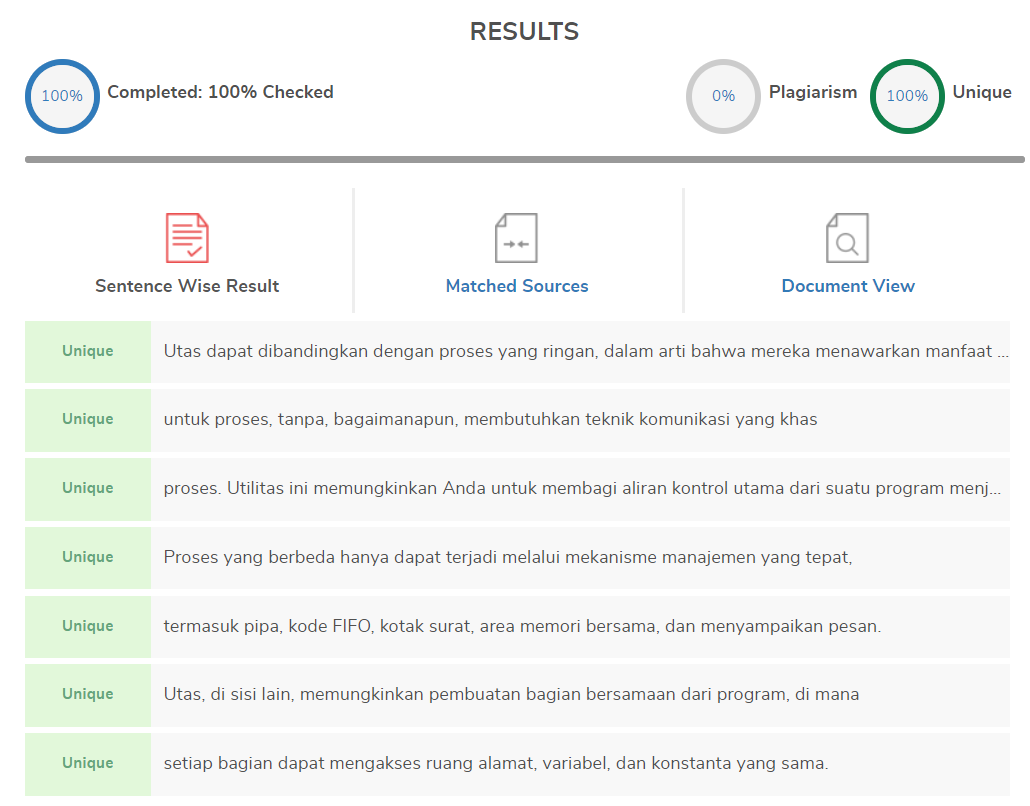
\includegraphics[width=4cm]{figures/kelompok1/1/dzihan/plagiat.PNG}
	\caption{Bukti Tidak Melakukan Plagiat Chapter 1}
\end{figure}


\section{1174021 - Muhammad Fahmi}
\subsection{Importing Libraries}
Libraries adalah kumpulan modul, tetapi istilah ini sering digunakan secara bergantian, terutama karena banyak library hanya terdiri dari satu modul, jadi jangan khawatir jika Anda mencampurnya. Library eksternal di impor dengan import [nama library]. Berikut ini sebuah contoh dari library random, yang menghasilkan integer secara acak.
\hfill\break
\lstinputlisting[firstline=29, lastline=32]{src/kelompok1/1174021/tugas1.py}
\hfill\break

	\begin{figure}[H]
		\centering
		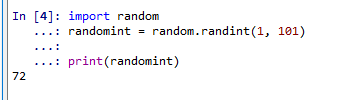
\includegraphics[width=4cm]{figures/kelompok1/1/1174021/tugas1/materi/2.PNG}
		\caption{Importing Libraries}
	\end{figure}

\subsection{Managing Files}
Managing files berfungsi untuk memungkinkan kita berinteraksi dengan sistem file, Python menyediakan kita dengan fungsi terbuka builtin. Fungsi ini dapat dipanggil untuk membuka file dan mengembalikan file objek. Itu
yang terakhir memungkinkan kita untuk melakukan berbagai operasi pada file, seperti membaca dan menulis. Setelah kita selesai berinteraksi dengan file, akhirnya kita harus ingat untuk menutupnya menggunakan metode file.close
\hfill\break
\lstinputlisting[firstline=36, lastline=45]{src/kelompok1/1174021/tugas1.py}
\hfill\break

	\begin{figure}[H]
		\centering
		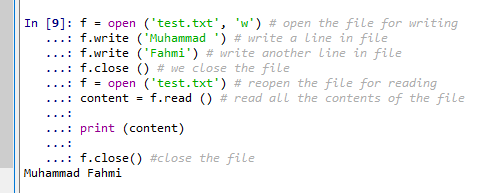
\includegraphics[width=4cm]{figures/kelompok1/1/1174021/tugas1/materi/3.PNG}
		\caption{Managing Files}
	\end{figure}

\subsection{List Comprehensions}
List comprehensions adalah alat yang ampuh untuk membuat dan memanipulasi daftar. Mereka terdiri dari ekspresi yang diikuti oleh untuk klausa dan kemudian diikuti oleh nol, atau lebih, jika klausa. Sintaksnya ialah expression for item in list. Kemudian, lakukan hal berikut:
\hfill\break
\lstinputlisting[firstline=49, lastline=56]{src/kelompok1/1174021/tugas1.py}
\hfill\break

	\begin{figure}[H]
		\centering
		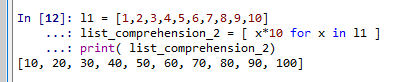
\includegraphics[width=4cm]{figures/kelompok1/1/1174021/tugas1/materi/41.PNG}
		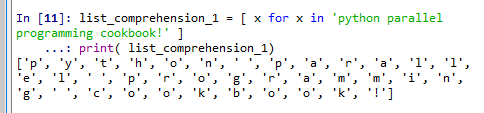
\includegraphics[width=4cm]{figures/kelompok1/1/1174021/tugas1/materi/42.PNG}
		\caption{List Comprehensions}
	\end{figure}

\subsection{Running Python Scripts}
Untuk menjalankan skrip Python, cukup panggil juru bahasa Python diikuti oleh skrip nama, dalam hal ini, mypythonscript.py. Atau, jika kita berada di direktori kerja yang berbeda, kemudian gunakan alamat lengkapnya:
\hfill\break
\lstinputlisting[firstline=58, lastline=60]{src/kelompok1/1174021/tugas1.py}
\hfill\break
Mulai sekarang, untuk setiap permintaan skrip Python, kita akan menggunakan
notasi sebelumnya; yaitu, python, diikuti oleh scriptname.py,
dengan asumsi bahwa direktori dari mana juru bahasa Python diluncurkan
adalah di mana skrip yang akan dieksekusi berada. Untuk memudahkan kita buat file python yang bernama mypythonscript.py, dengan codingan sebagai berikut, lalu buka cmd atau anaconda prompt untuk memanggil file python tersebut.
\hfill\break
\lstinputlisting[firstline=53, lastline=56]{src/kelompok1/1174021/tugas1.py}
\hfill\break

	\begin{figure}[H]
		\centering
		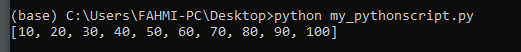
\includegraphics[width=4cm]{figures/kelompok1/1/1174021/tugas1/materi/5.PNG}
		\caption{Running Python Scripts}
	\end{figure}

\subsection{Installing Python packages using pip}
Pip adalah alat yang memungkinkan kita untuk mencari, mengunduh, dan menginstal paket Python yang ditemukan di Internet Python Package Index, yang merupakan repositori yang berisi puluhan ribu paket ditulis dengan Python. Ini juga memungkinkan kita untuk mengelola paket yang kita miliki diunduh, memungkinkan kami untuk memperbarui atau menghapusnya.
\subsubsection{Installing Pip}
Pip sudah termasuk dalam versi Python 3.4 dan 2.7.9. Untuk memeriksa apakah alat ini sudah terpasang, kita dapat menjalankan perintah berikut
\hfill\break

	\begin{figure}[H]
		\centering
		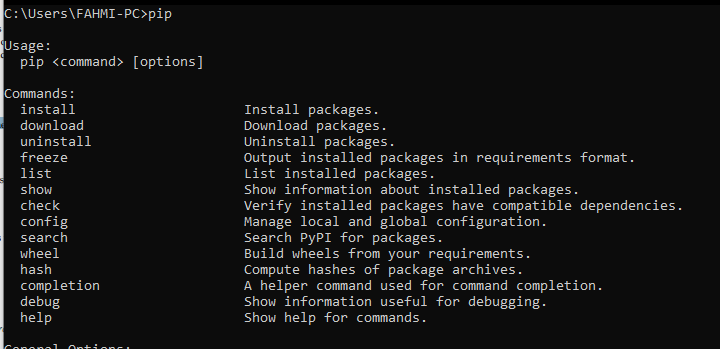
\includegraphics[width=4cm]{figures/kelompok1/1/1174021/tugas1/materi/61.PNG}
		\caption{Installing Pip}
	\end{figure}

\subsubsection{Updating Pip}
Disarankan juga untuk memeriksa bahwa versi Pip yang Anda gunakan selalu terkini. Untuk perbarui itu, kita bisa menggunakan perintah berikut:
\hfill\break

	\begin{figure}[H]
		\centering
		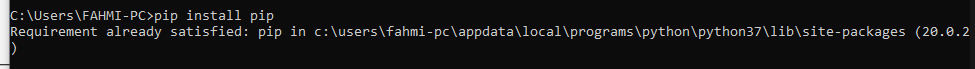
\includegraphics[width=4cm]{figures/kelompok1/1/1174021/tugas1/materi/62.PNG}
		\caption{Updating Pip}
	\end{figure}

\subsubsection{Using Pip}
Pip mendukung serangkaian perintah yang memungkinkan, antara lain, untuk mencari, mengunduh, instal, perbarui, dan hapus library. Untuk menginstal library atau modul pada python, contoh disini kita menginstall matplotlib, jalankan perintah berikut :
\hfill\break

	\begin{figure}[H]
		\centering
		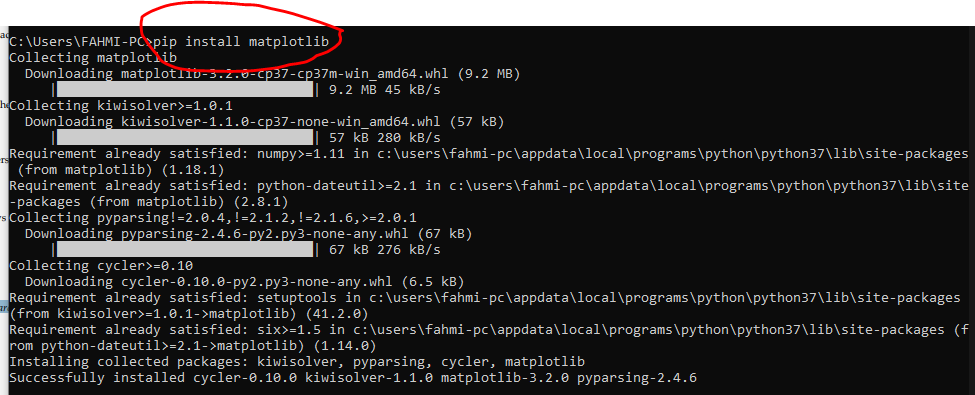
\includegraphics[width=4cm]{figures/kelompok1/1/1174021/tugas1/materi/63.PNG}
		\caption{Using Pip}
	\end{figure}
	
\subsection{Penanganan Error}
\begin{enumerate}
	\item ScreenShoot Error
	\begin{figure}[H]
		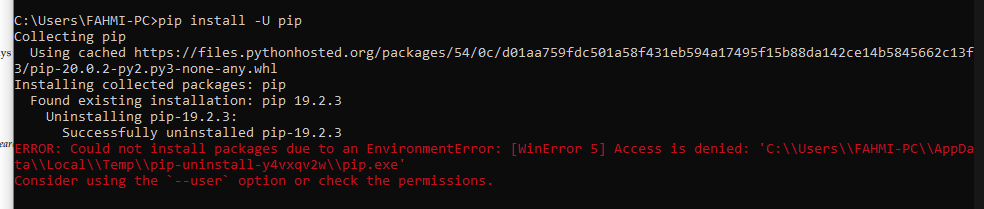
\includegraphics[width=4cm]{figures/kelompok1/1/1174021/tugas1/error/1.PNG}
		\centering
		\caption{Could not install packages}
	\end{figure}
	\item Cara Penanganan Error
	Error terdapat pada penamaan kesalahan install packages, seharusnya menghapuskan -U.
\end{enumerate}

\subsection{Bukti Tidak Plagiat}
\begin{figure}[H]
\centering
	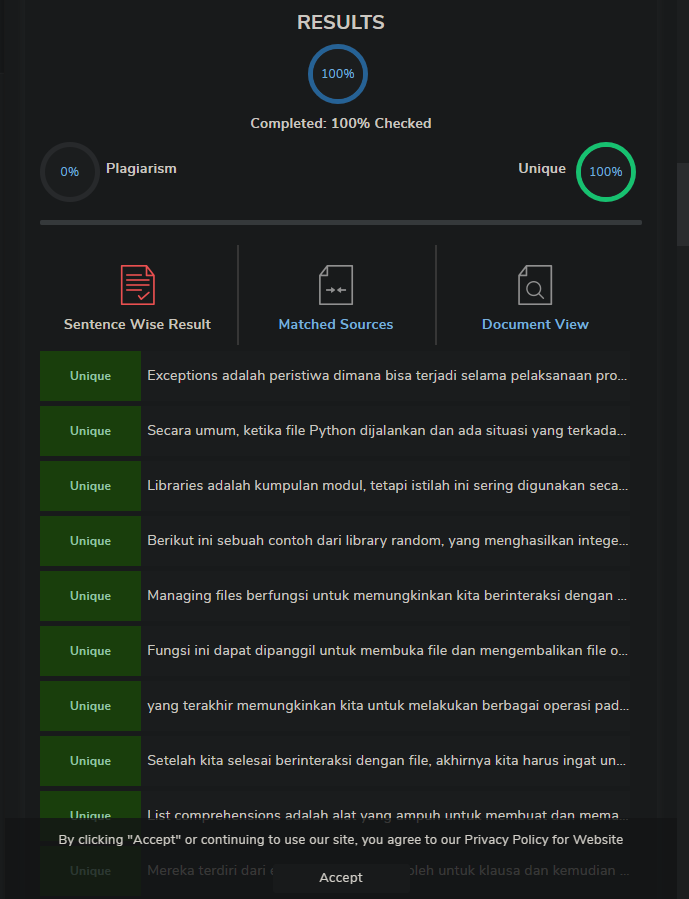
\includegraphics[width=4cm]{figures/kelompok1/1/1174021/tugas1/buktiplagiat/1.PNG}
	\caption{Bukti Tidak Melakukan Plagiat Chapter 1}
\end{figure}

\section{1174031 - Muhammad Tomy Nur Maulidy}
\subsection{Memperkenalkan pemrograman paralel Python}
	Python menyediakan banyak pustaka dan kerangka kerja yang memfasilitasi kinerja tinggi
perhitungan. Namun, melakukan pemrograman paralel dengan Python bisa sangat berbahaya
karena Global Interpreter Lock (GIL).
Bahkan, interpreter Python yang paling luas dan banyak digunakan, CPython, dikembangkan di
bahasa pemrograman C. Penerjemah CPython membutuhkan GIL untuk keamanan thread
operasi. Penggunaan GIL menyiratkan bahwa Anda akan menemukan kunci global ketika Anda mencoba
untuk mengakses objek Python yang ada di dalam utas. Dan hanya satu utas dalam satu waktu yang bisa
memperoleh kunci untuk objek Python atau API C.
Untungnya, masalahnya tidak terlalu serius, karena, di luar ranah GIL, kita bisa leluasa menggunakannya
paralelisme. Kategori ini mencakup semua topik yang akan kita bahas dalam bab-bab berikutnya,
termasuk multiprocessing, komputasi terdistribusi, dan komputasi GPU.
Jadi, Python tidak benar-benar multithreaded. Tapi apa itu utas? Apa itu proses? Dalam
bagian berikut, kami akan memperkenalkan dua konsep dasar ini dan bagaimana mereka
ditangani oleh bahasa pemrograman Python.
\subsection{Proses dan utas}
Utas dapat dibandingkan dengan proses yang ringan, dalam arti bahwa mereka menawarkan manfaat yang serupa untuk proses, tanpa, bagaimanapun, membutuhkan teknik komunikasi yang khas proses. Utilitas ini memungkinkan Anda untuk membagi aliran kontrol utama dari suatu program menjadi beberapa secara bersamaan menjalankan aliran kontrol. Sebagai gantinya, proses memiliki ruang pengalamatan sendiri dan sumber daya mereka sendiri. Kemudian komunikasi antar bagian kode berjalan Proses yang berbeda hanya dapat terjadi melalui mekanisme manajemen yang tepat, termasuk pipa, kode FIFO, kotak surat, area memori bersama, dan menyampaikan pesan. Utas, di sisi lain, memungkinkan pembuatan bagian bersamaan dari program, di mana setiap bagian dapat mengakses ruang alamat, variabel, dan konstanta yang sama.
\subsection{Praktek}
\begin{enumerate}
	\item do something
    \lstinputlisting[firstline=8, lastline=12]{src/kelompok1/do_something.py}
	\hfill\break
	\item serial test
	\hfill\break
	\lstinputlisting[firstline=8, lastline=22]{src/kelompok1/serial_test.py}
	\item multithreading test
	\hfill\break
	\lstinputlisting[firstline=8, lastline=30]{src/kelompok1/multithreading_test.py}
	\item multiprocessing test
	\hfill\break
	\lstinputlisting[firstline=8, lastline=30]{src/kelompok1/multiprocessing_testpy.py}
\end{enumerate}
\subsection{Percobaan}
\begin{enumerate}
	\item Menjalankan Serial Test
	\begin{figure}[H]
		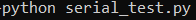
\includegraphics[width=4cm]{figures/kelompok1/1/tomy/test1.PNG}
		\centering
		\caption{Menjalankan Serial Test}
	\end{figure}
	\begin{figure}[H]
		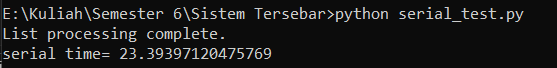
\includegraphics[width=4cm]{figures/kelompok1/1/tomy/hasil1.PNG}
		\centering
		\caption{Hasil Serial Test}
	\end{figure}
    \item Menjalankan Multithreading Test
	\begin{figure}[H]
		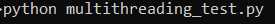
\includegraphics[width=4cm]{figures/kelompok1/1/tomy/test2.PNG}
		\centering
		\caption{Menjalankan Multithreading Test}
	\end{figure}
	\begin{figure}[H]
		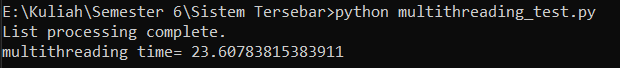
\includegraphics[width=4cm]{figures/kelompok1/1/tomy/hasil2.PNG}
		\centering
		\caption{Hasil Multithreading Test}
	\end{figure}
    \item Menjalankan Multiprocessing Test
	\begin{figure}[H]
		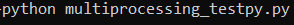
\includegraphics[width=4cm]{figures/kelompok1/1/tomy/test3.PNG}
		\centering
		\caption{Menjalankan Multiprocessing Test}
	\end{figure}
	\begin{figure}[H]
		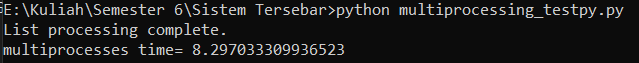
\includegraphics[width=4cm]{figures/kelompok1/1/tomy/hasil3.PNG}
		\centering
		\caption{Hasil Multiprocessing Test}
	\end{figure}
\end{enumerate}
\subsection{Bukti Tidak Plagiat}
\begin{figure}[H]
	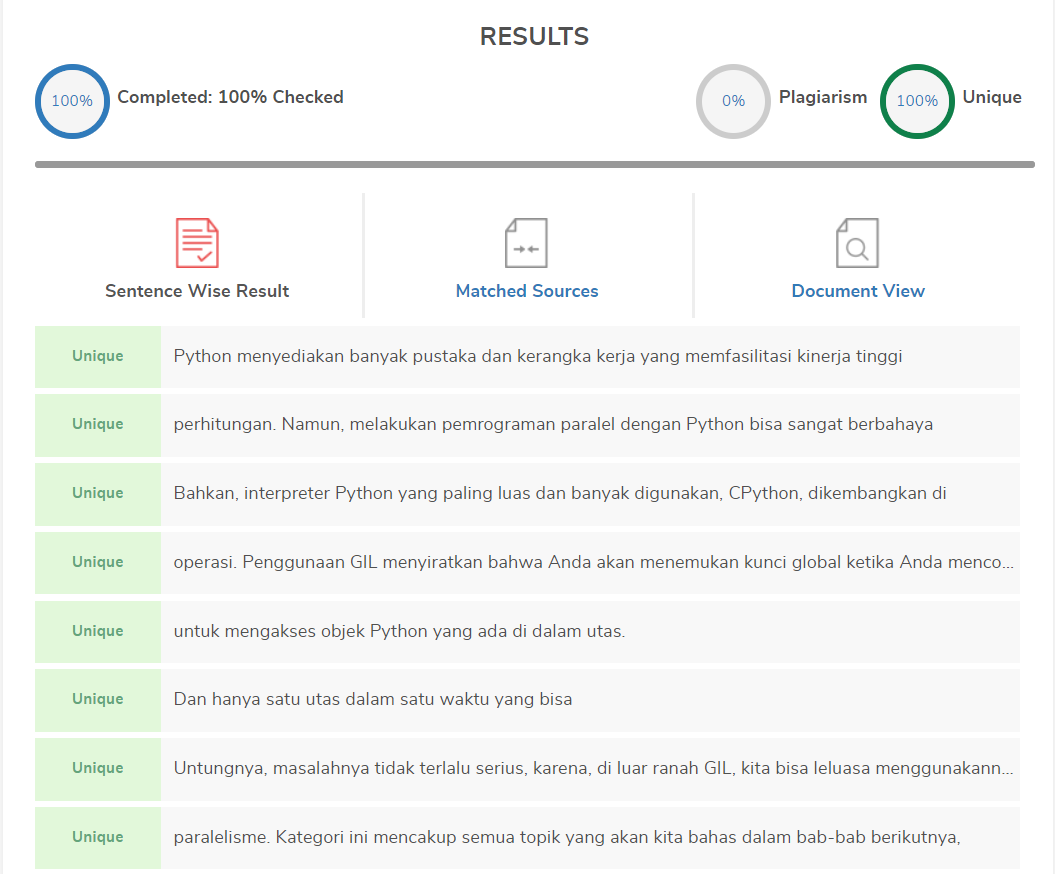
\includegraphics[width=4cm]{figures/kelompok1/1/tomy/plagiat_tomy_1.PNG}
	\centering
	\caption{Bukti Tidak Melakukan Plagiat 1}
    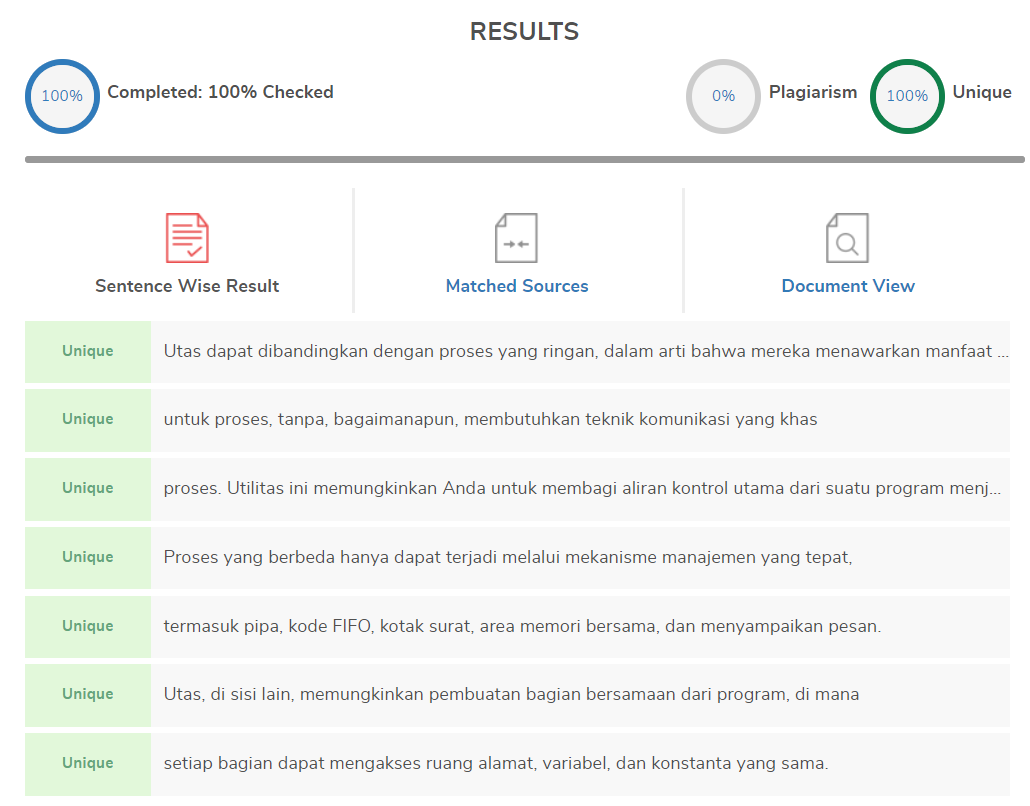
\includegraphics[width=4cm]{figures/kelompok1/1/tomy/plagiat_tomy_2.PNG}
	\centering
	\caption{Bukti Tidak Melakukan Plagiat 2}
\end{figure}
